% !TEX TS-program = xelatex
% !TEX encoding = UTF-8
% !Mode:: "TeX:UTF-8"

\documentclass[onecolumn,oneside]{SUSTechHomework}

\usepackage{float}

\author{胡玉斌}
\sid{11712121}

\title{Lab 11}
\coursecode{CS315}
\coursename{Computer Security}

\begin{document}
  \maketitle

  \section*{Task 1}
  Posting a Malicious Message to Display an Alert Window

  \begin{figure}[H]
    \centering
    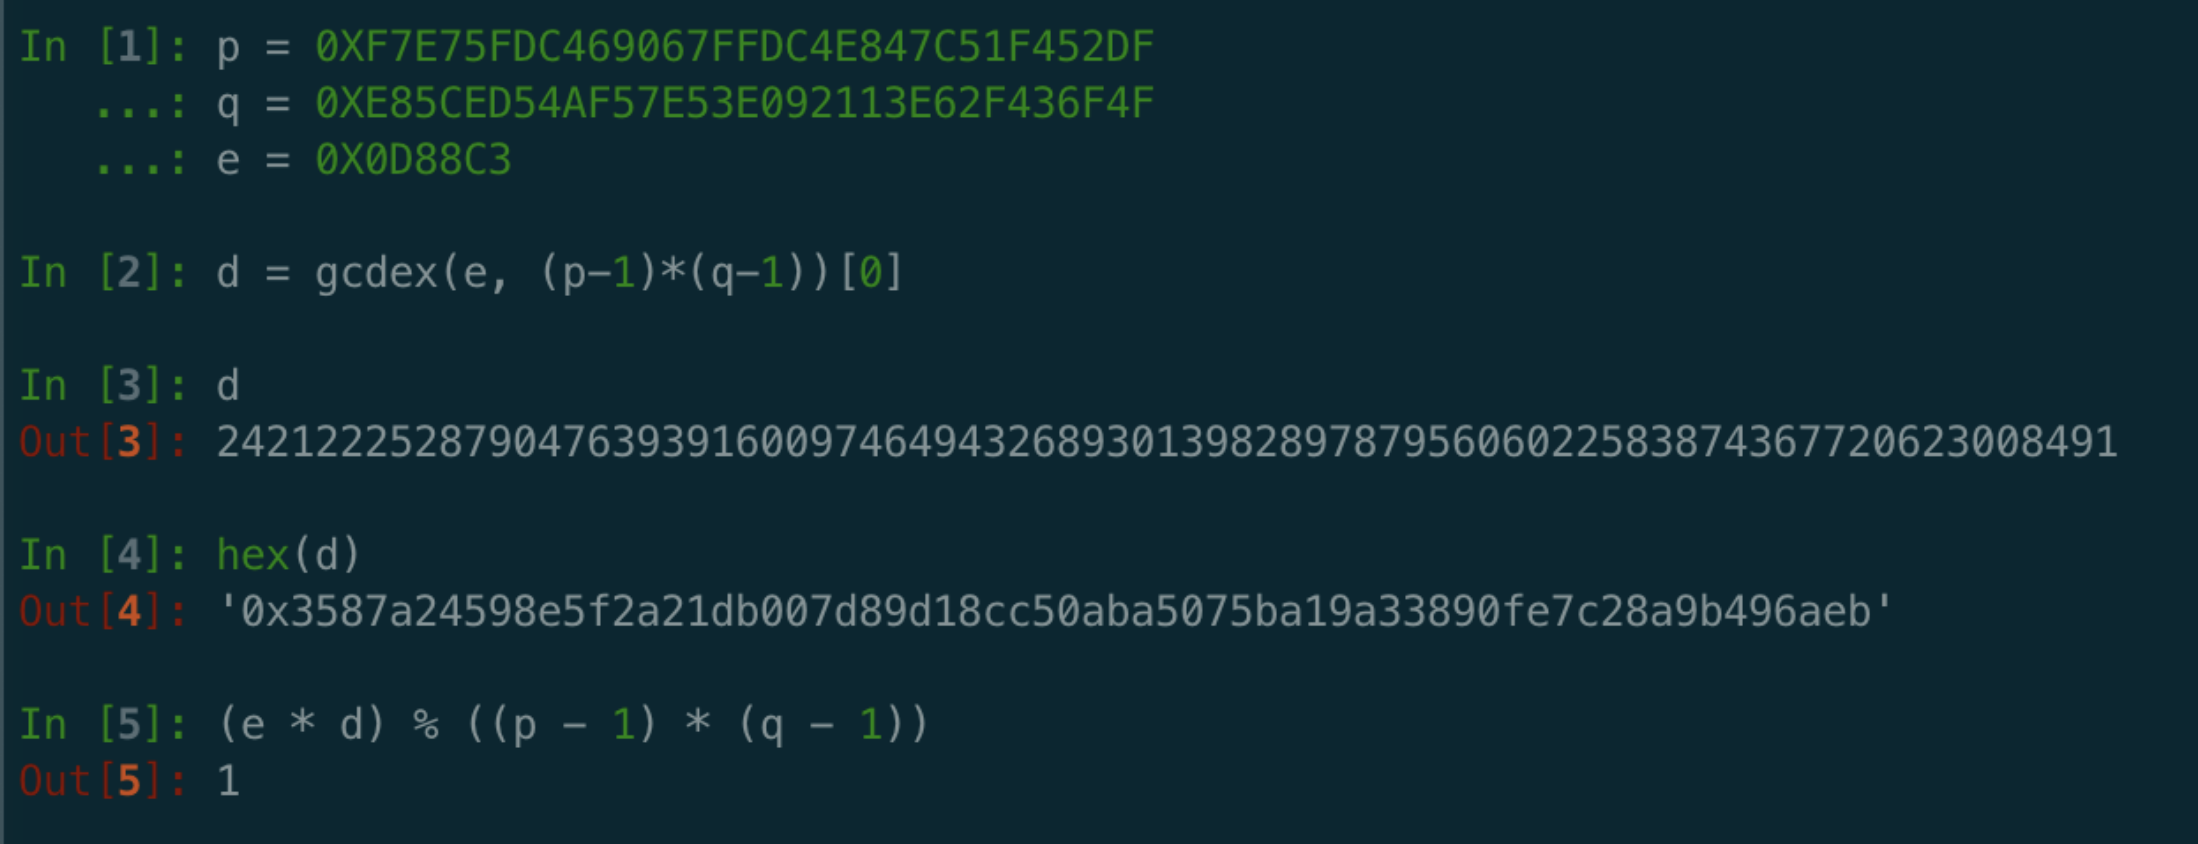
\includegraphics[width=0.85\textwidth]{img/task1_1.png}
    \caption{embed JavaScript code}
  \end{figure}

  \begin{figure}[H]
    \centering
    \includegraphics[width=0.85\textwidth]{img/task1_2.png}
    \caption{XSS}
  \end{figure}

  \section*{Task 2}
  Posting a Malicious Message to Display Cookies

  \begin{figure}[H]
    \centering
    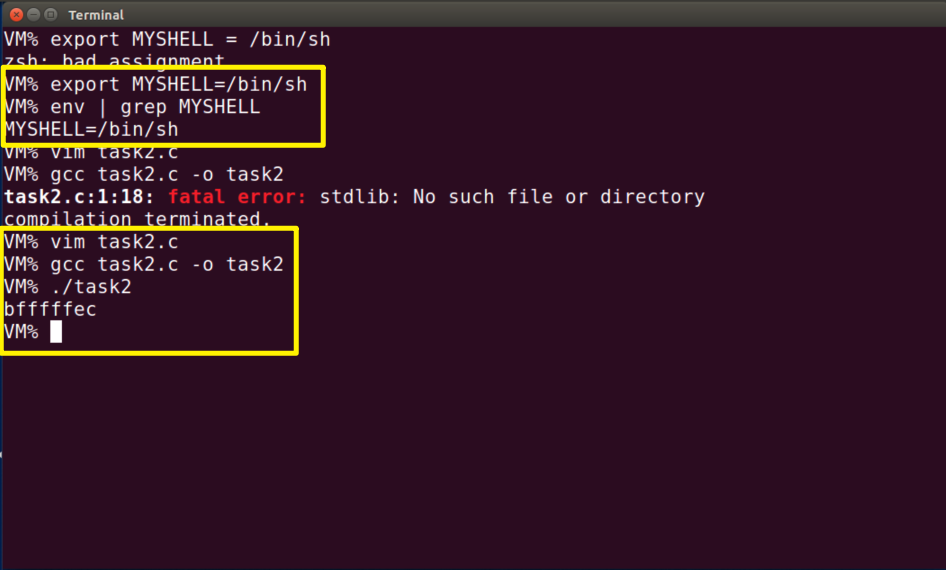
\includegraphics[width=0.85\textwidth]{img/task2_1.png}
    \caption{embed JavaScript code}
  \end{figure}

  \begin{figure}[H]
    \centering
    \includegraphics[width=0.85\textwidth]{img/task2_2.png}
    \caption{cookie}
  \end{figure}

  \section*{Task 3}
  Stealing Cookies from the Victim’s Machine

  \begin{figure}[H]
    \centering
    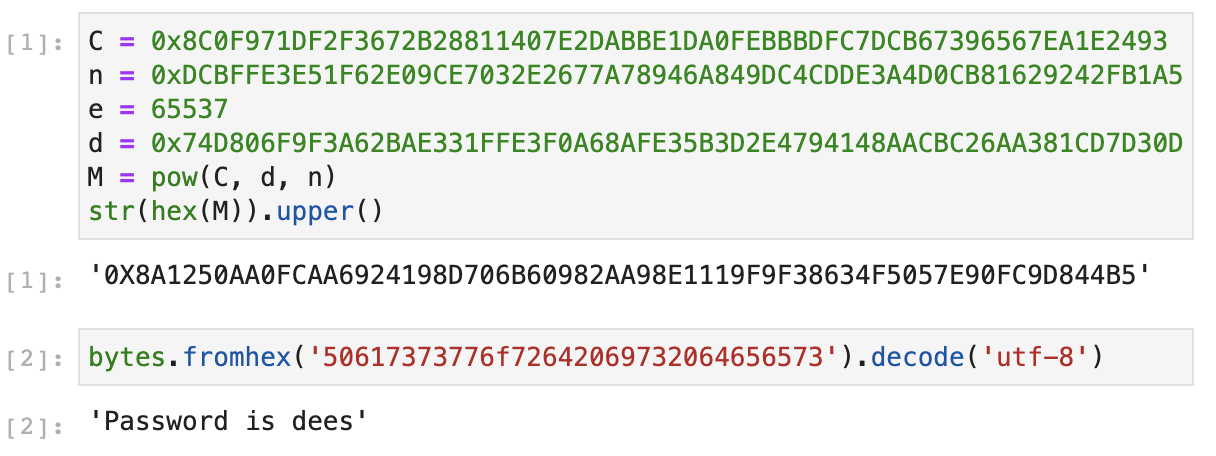
\includegraphics[width=0.85\textwidth]{img/task3_1.png}
    \caption{embed JavaScript code} 
  \end{figure}

  \begin{figure}[H]
    \centering
    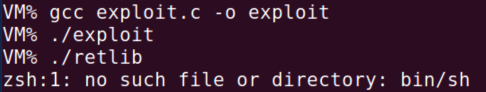
\includegraphics[width=0.85\textwidth]{img/task3_2.png}
    \caption{nc -l 5555 -v}
  \end{figure}

  \section*{Task 4}
  Becoming the Victim’s Friend

  \begin{figure}[H]
    \centering
    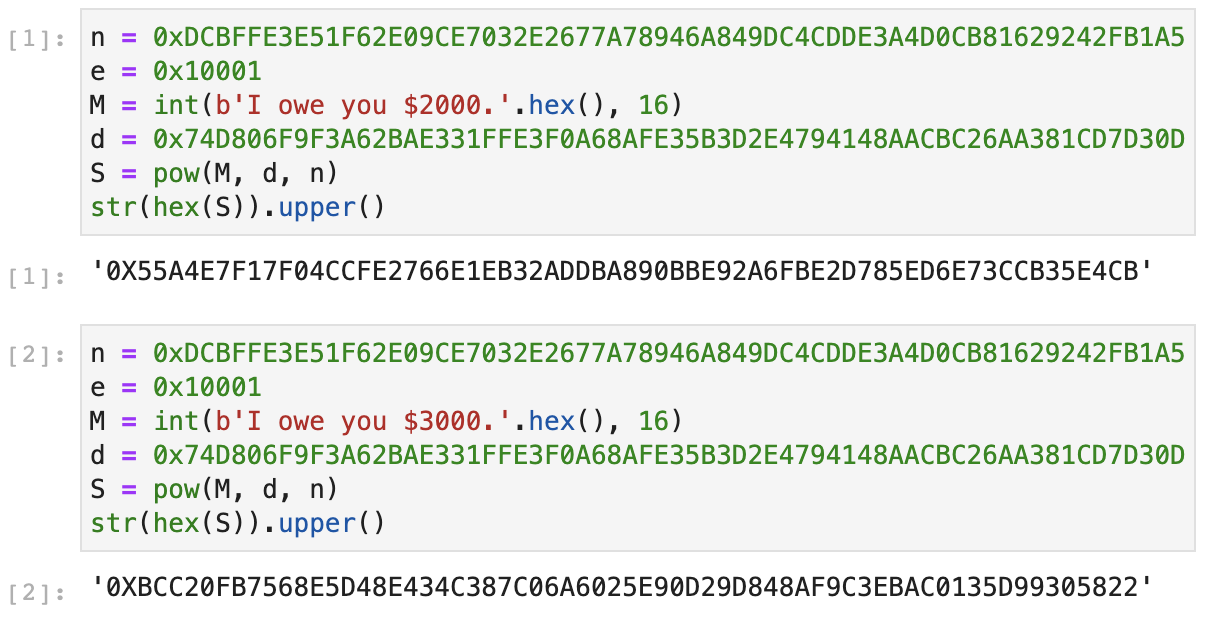
\includegraphics[width=0.85\textwidth]{img/task4_1.png}
    \caption{embed JavaScript code} 
  \end{figure}

  \begin{figure}[H]
    \centering
    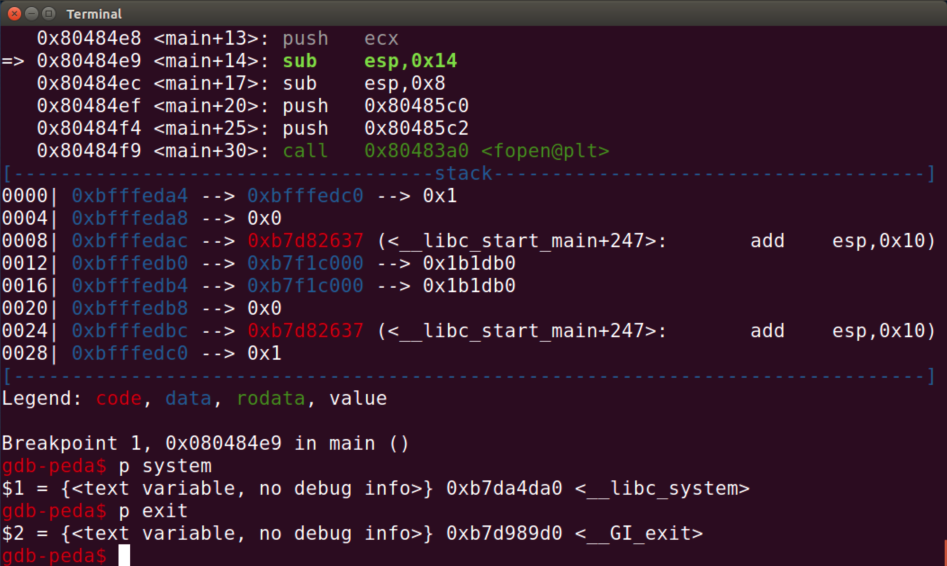
\includegraphics[width=0.85\textwidth]{img/task4_2.png}
    \caption{add friends}
  \end{figure}

    \subsection*{Q1}

      \verb|ts| and \verb|token| are used for authentication. So that the operate can be succeed.

    \subsection*{Q2}

      No, we cannot launch a successful attack, because we cannot have a HTML entry in \verb|"About me"|

  \section*{Task 5}
  Modifying the Victim’s Profile

  \begin{figure}[H]
    \centering
    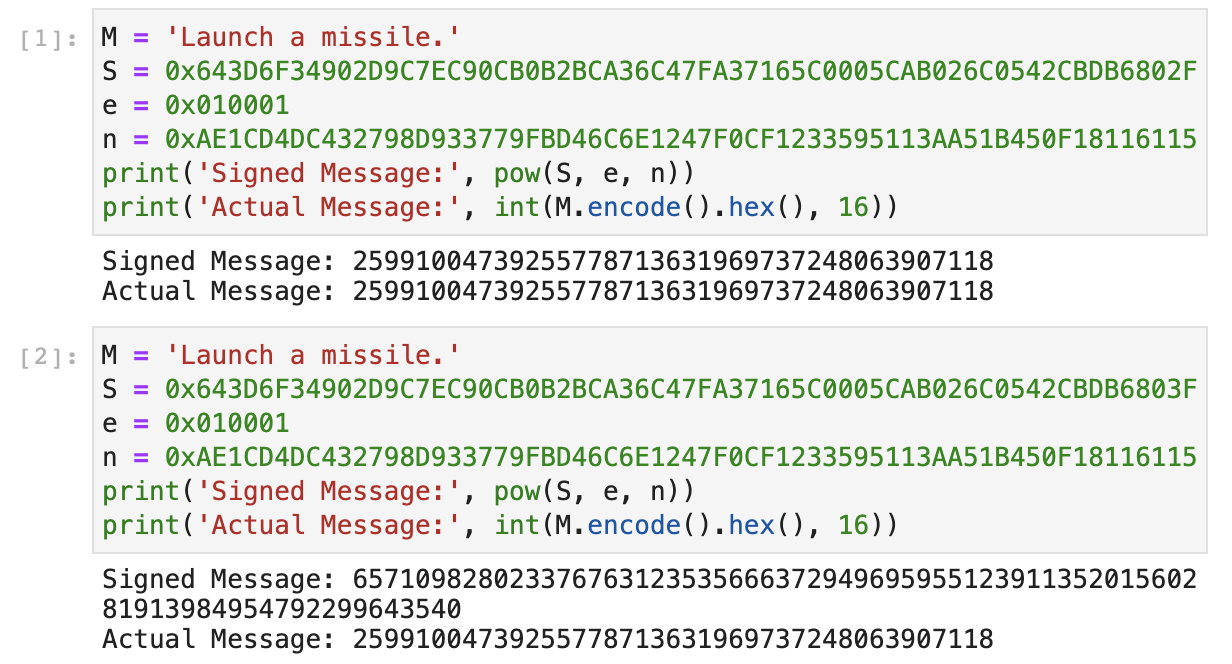
\includegraphics[width=0.85\textwidth]{img/task5_1.png}
    \caption{embed JavaScript code} 
  \end{figure}

  \begin{figure}[H]
    \centering
    \includegraphics[width=0.85\textwidth]{img/task5_2.png}
    \caption{modify profile}
  \end{figure}

    \subsection*{Q3}

      This line is needed, otherwise Samy will modify his own profile and overwrite the JavaScript code.

  \section*{Task 6}
  Writing a Self-Propagating XSS Worm

  \begin{figure}[H]
    \centering
    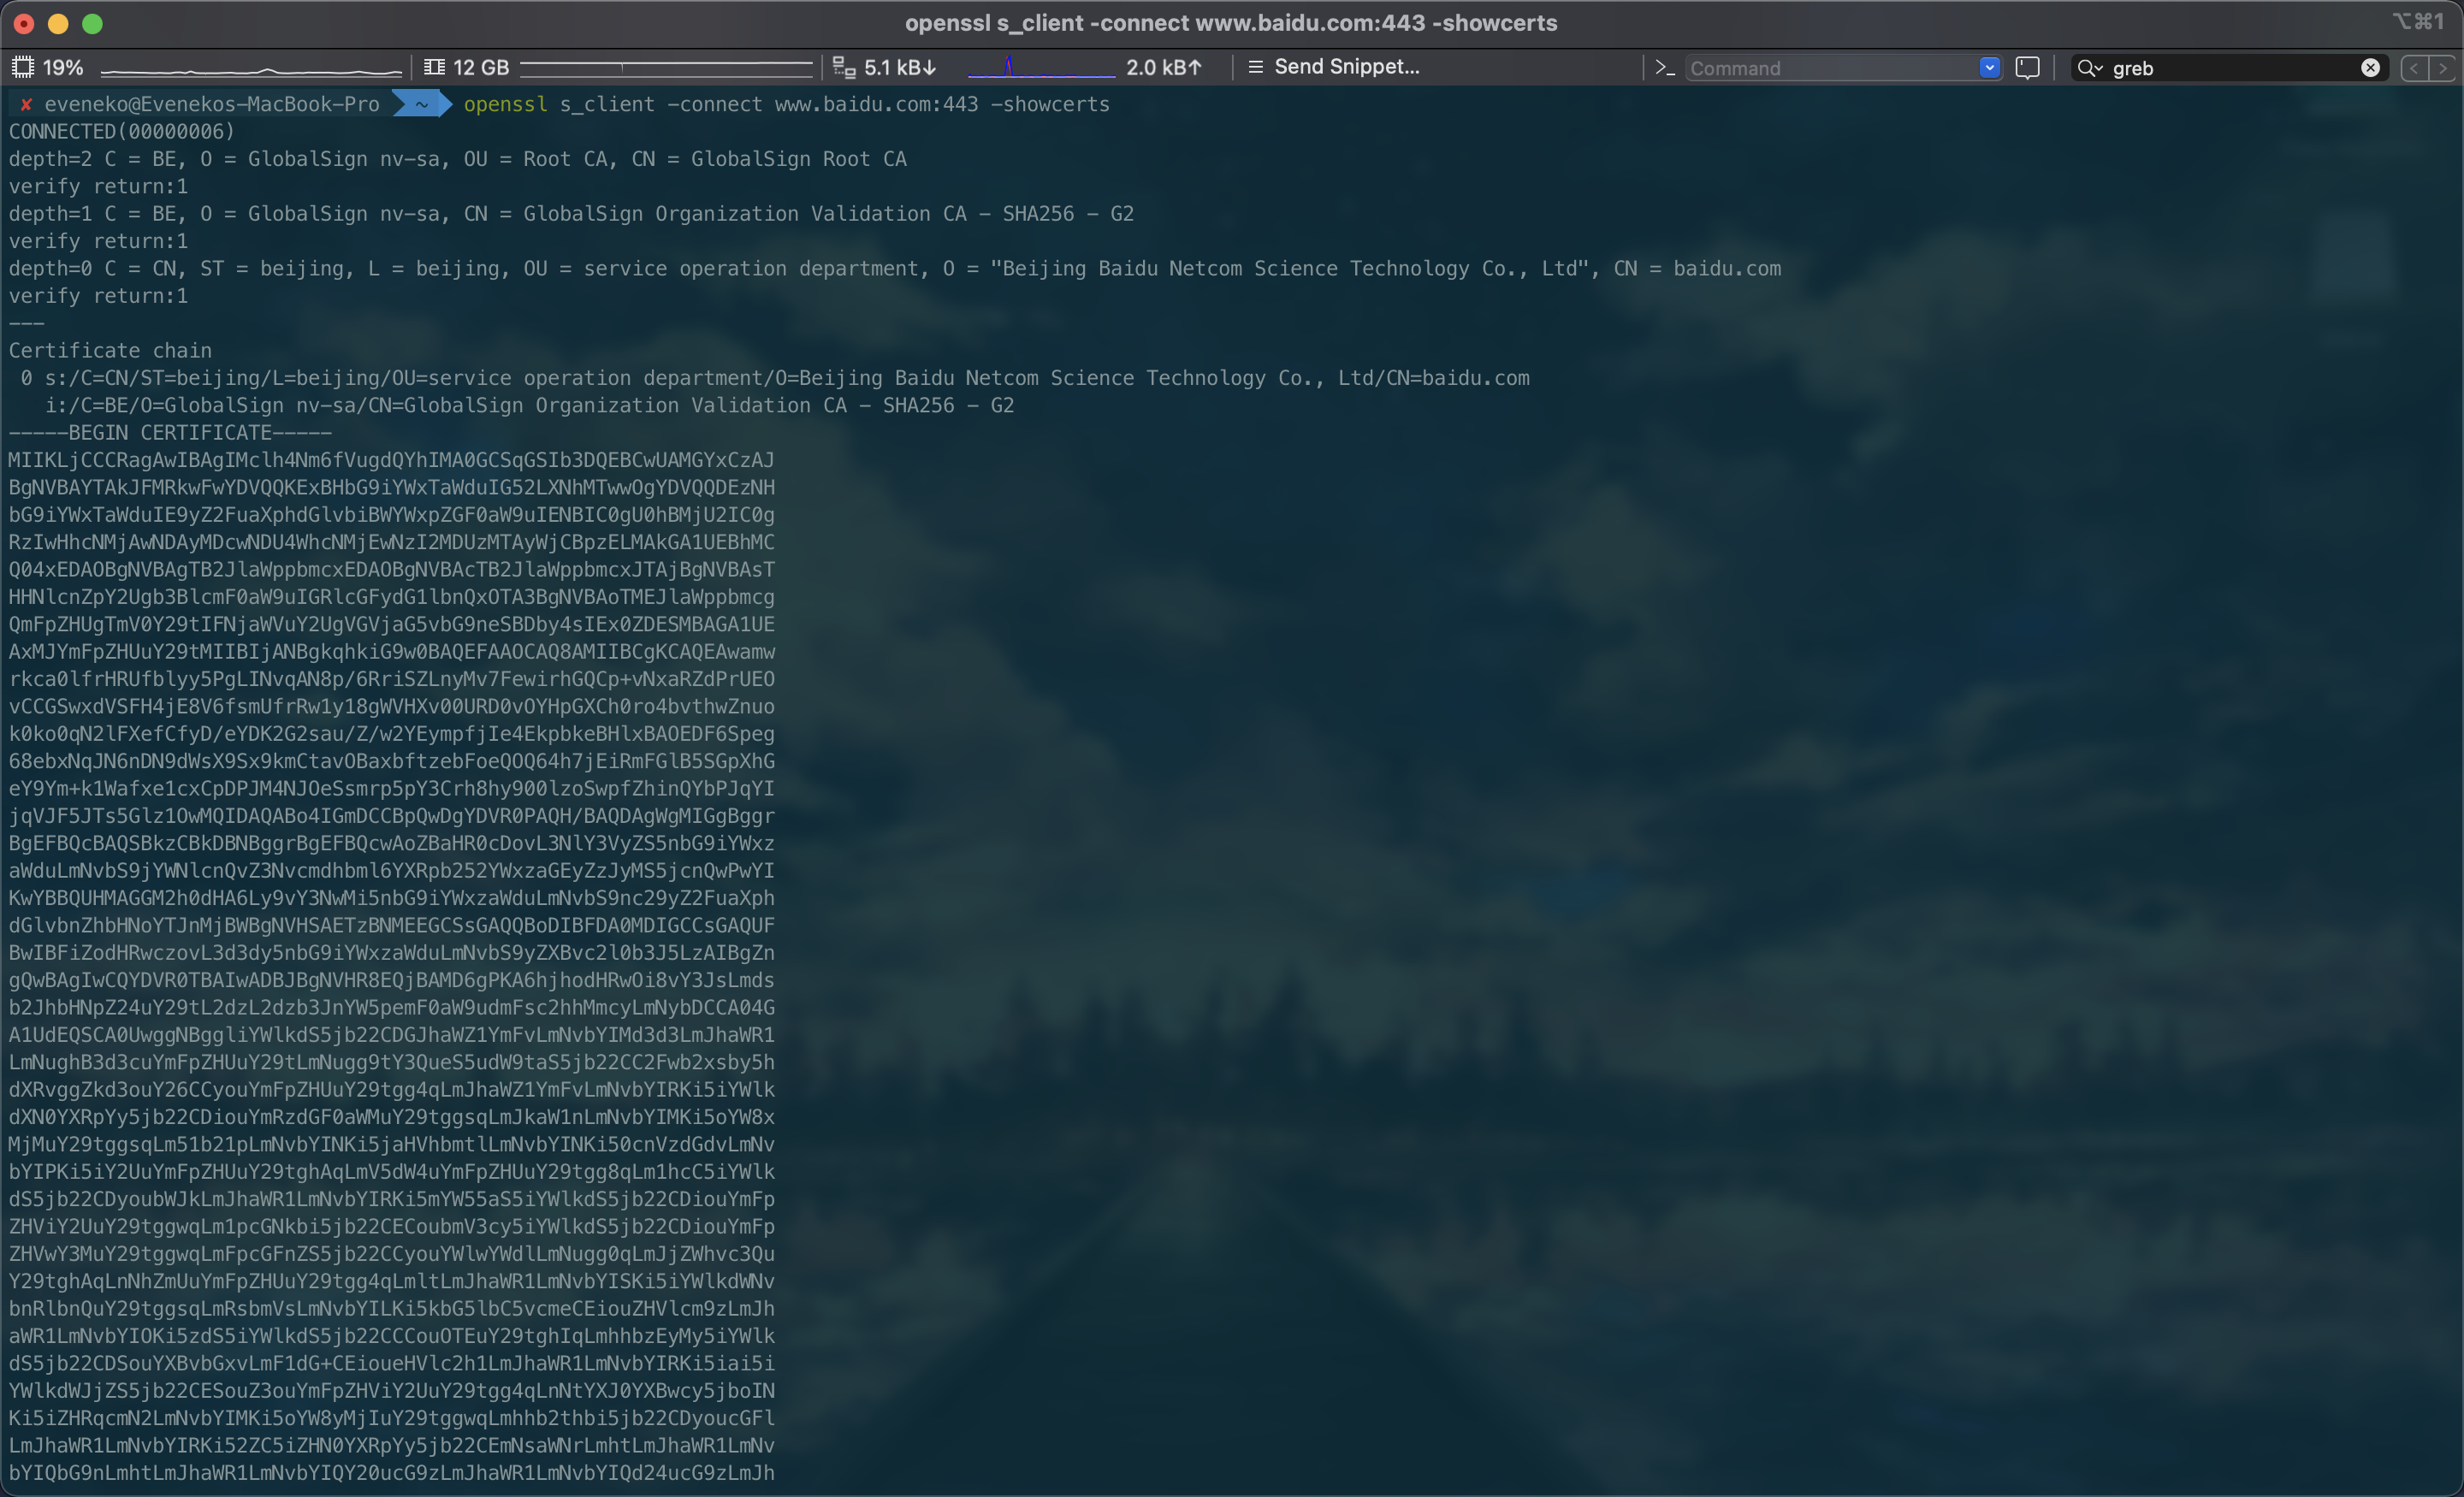
\includegraphics[width=0.85\textwidth]{img/task6_1.png}
    \caption{XSS Worm} 
  \end{figure}

  \begin{figure}[H]
    \centering
    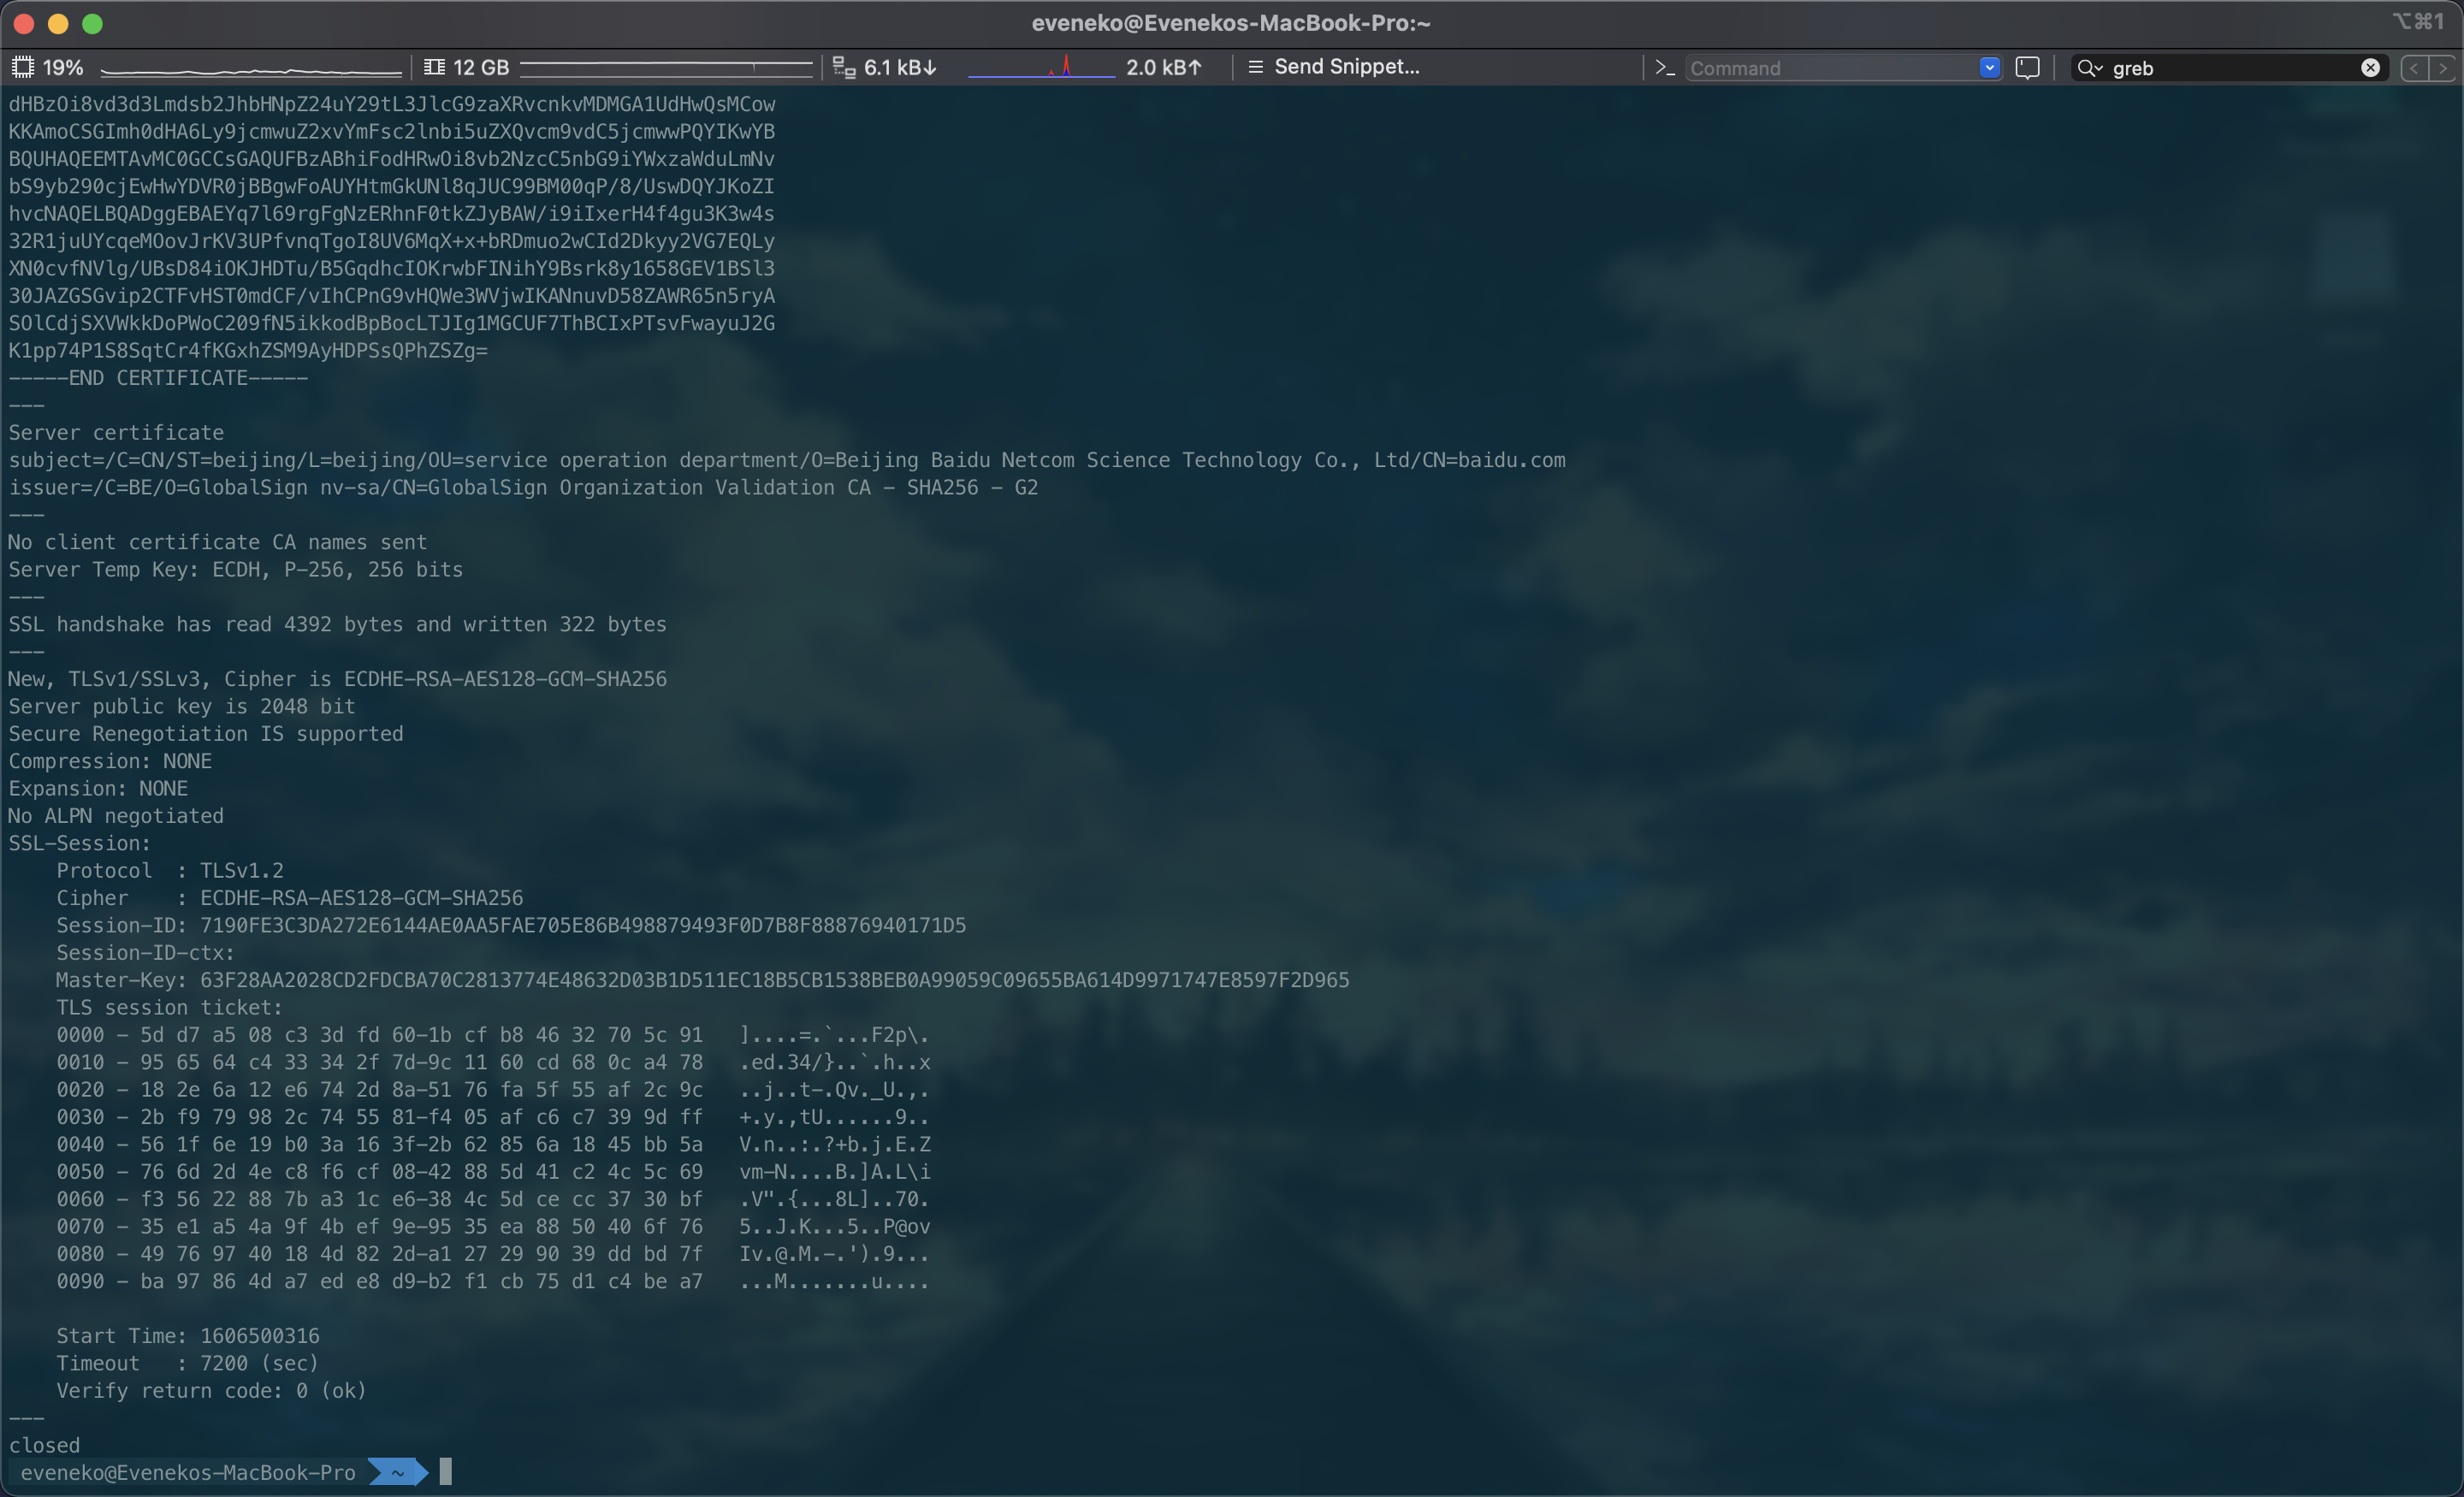
\includegraphics[width=0.85\textwidth]{img/task6_2.png}
    \caption{XSS Worme}
  \end{figure}

  \begin{figure}[H]
    \centering
    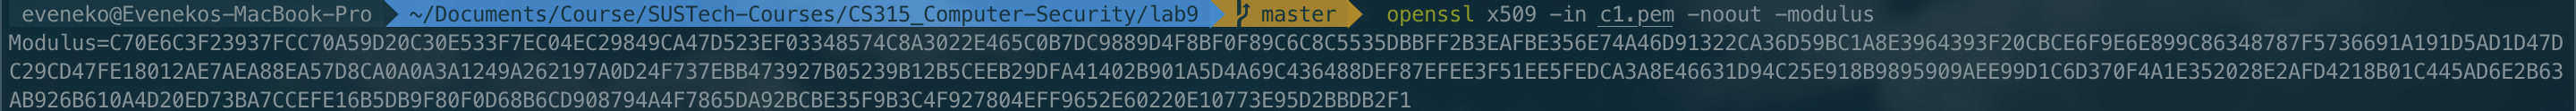
\includegraphics[width=0.85\textwidth]{img/task6_3.png}
    \caption{modify profile}
  \end{figure}

  \section*{Task 7}
  Countermeasures

  \begin{itemize}
    \item Enabling HTMLawed, the HTML tags are removed in editors
    \item Uncommenting htmlspecialchars , the attack no longer works.
  \end{itemize}

  \begin{figure}[H]
    \centering
    \includegraphics[width=0.85\textwidth]{img/task7_1.png}
    \caption{Countermeasures} 
  \end{figure}

\end{document}
